\documentclass[a4paper]{scrartcl}

\usepackage[
fancytheorems, 
fancyproofs, 
noindent, 
%  spacingfix,  
]{adam}

\usepackage{tikz}
\usepackage{cancel}


\title{Variational Principles}
\author{Adam Kelly (\texttt{ak2316@cam.ac.uk})}
\date{\today, to Lecture 5}


\allowdisplaybreaks

\begin{document}

\maketitle

From finding geodesics to expressing the fundamental laws of nature, variational principles and the calculus of variations arise naturally in pure \& applied mathematics, and theoretical physics.
Here, we will study such ideas, with the underlying goal of considering problems involving minimizing (or maximizing) quantities that depend on an entire function. 

This article constitutes my notes for the `Variational Principles' course, held in Easter 2021 at Cambridge. These notes are \emph{not a transcription of the lectures}, and differ significantly in quite a few areas. Still, all lectured material should be covered.

% {\color{purple}Currently up to lecture 1.}

\tableofcontents

\section{Introduction}


% Lecture 1

We will begin our study of variational principles by getting a feel for the type of problems that we care about. 
As a field, the study of variational principles can be traced back to a single problem, posed by Johann Bernoulli in 1696. It is there that we will begin.

\subsection{A Motivating Problem -- The Brachistochrone}

One of the earliest problems in the calculus of variations is the \vocab{Brachistochrone} problem.

\begin{example}[Brachistochrone]
	Consider a particle sliding on a wire between two fixed points $A$ and $B$, under the influence of gravity. Which shape of the wire will give the shortest travel time, when the particle starts from rest?
\end{example}

It is not immediately obvious what the answer to this problem is. We won't solve it right now, but we can still can take some steps in the right direction. We first setup a coordinate system, setting $A$ to be the origin, and $B$ to be some point $(x_2, y_2)$.

\begin{center}
	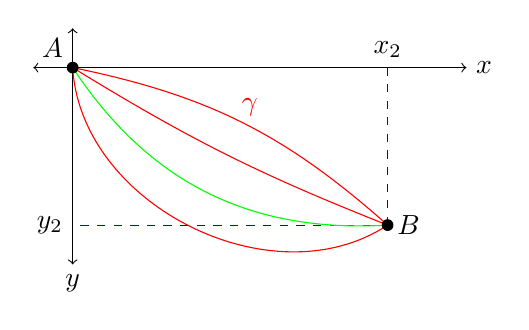
\begin{tikzpicture}
		\coordinate (origin) at (0,0);
		\coordinate (b) at (4.0, -2.0);
		
		% \filldraw[color=blue!80, fill=blue!2] (z1) circle (0.7);

		% draw axes
		\draw [<->] (-0.5, 0) -- (5.0, 0) node [right] {$x$};
		\draw [<->] (0, 0.5) -- (0, -2.5) node [below] {$y$};
	
		\draw [dashed, blue] (b) -- (4.0, 0) node [black, above] {$x_2$};
		\draw [dashed, blue] (b) -- (0, -2.0) node [black, left] {$y_2$};

		% draw some paths between A and B
		\draw [green] (origin) to [bend right=30] (b);
		\draw [red] (origin) to [bend right=60] (b);
		\draw [red] (origin) to [bend right=5] (b);
		\draw [red] (origin) to [bend left=15] (b);

		\draw (2.25, -0.5) node [red] {$\gamma$};
		% \draw plot [smooth, red] coordinates {(0,0) (2.0, -1.2) (4.0, -2.0))};

		% draw the points A and B
		\node at (b)[circle,fill,inner sep=1.5pt]{};
		\draw (b) node [right] {$B$};

		\node at (origin)[circle,fill,inner sep=1.5pt]{};
		\draw (origin) node [above left] {$A$};

		% draw vectors
		% \draw [->] (origin) -- (z1) node [anchor=south west] {$c$};
		% \draw [dashed] (1, 1.25) -- (0.3, 1.25) node [pos=0.5, anchor=south] {$\rho$};
		\end{tikzpicture}
\end{center}

In this coordinate system, for a given curve $\gamma$, we can write down the travel time 
$$
T = \int_\gamma \dd t = \int_\gamma \frac{1}{v} \dd s,
$$
where $v$ is the velocity of the particle. Since the particle starts at $y = 0$, conservation of energy implies that 
\begin{align*}
	\frac{1}{2}m v^2 + mg y &= 0 \\
	\implies v &= \sqrt{-2gy}.
\end{align*}
Thus to solve our problem, we really want to minimize
$$
T[y] = \frac{1}{\sqrt{2g}} \int_0^{x_2} \frac{\sqrt{1 + (y')^2}}{\sqrt{-y}} \dd x,
$$
subject to $y$ being a smooth function with $y(0) = 0$, and $y(x_2) = y_2$.

\subsection{Problems of Interest}

Let's jump to another problem from pure mathematics, finding geodesics.

\begin{example}[Geodesic Problem]
	Find the shortest path $\gamma$ between two points on a surface $\Sigma$ (if one exists).
\end{example}


If $\Sigma$ is $\R^2$, we can again adopt a coordinate system, and try to find the shortest curve $\gamma$ between the two points $A = (x_1, y_1)$ and $B=(x_2, y_2)$.
To solve this problem, we really want to minimize
$$
D[y] = \int_{x_1}^{x_2} \sqrt{1 + (y')^2} \dd{x},
$$
subject to $y$ being a smooth function with $y(x_1) = y_1$ and $y(x_2) = y_2$.

Both of these problems have a similar flavour: we are trying the minimize or maximize something like
\begin{equation}\label{eq:functional}
	F[y] = \int_{x_1}^{x_2} f(x, y(x), y'(x)) \dd x, \tag{$*$}
\end{equation}
among all functions such that $y(x_1) = y_1$ and $y(x_2) = y_2$.
This quantity \eqref{eq:functional} is called a \vocab{functional}, that is, a function on the space of functions\footnote{In standard calculus, we usually consider functions which map numbers $\rightarrow$ numbers. In the calculus of variations, we consider \emph{functional} which map functions $\rightarrow$ numbers. An intuitive example is that of arc-length, which takes some curve and gives back a number corresponding to its length.}.

In this article, we are going to study the \emph{calculus of variations}, in which we will be finding extrema (minima, maxima, and saddle points) of functionals. 
We will start by looking back at and extending our knowledge of extrema in finite dimensions, before using this knowledge to approach problems involving functionals.

\begin{notation}
	Throughout this article, we will frequently refer to different spaces of functions. We will let $C(\R)$ be the space of continuous functions on $\R$, and $C^k(\R)$ be the space of functions with continuous $k$th derivative. We will also write $C_{(\alpha, \beta)}^k(\R)$ for the subset of functions $f$ with $f(\alpha) = f(\beta)$.
\end{notation}

% Lecture 2

\section{Calculus for Functions on \texorpdfstring{$\R^n$}{R-n}}

For this section, we are going to consider a function $f \in C^2(\R^n)$, that is, $f: \R^n \rightarrow \R$, with continuous second derivative.

\subsection{Stationary Points}

Recall the definition of a stationary point for a function $f \in C^2(\R^n)$.

\begin{definition}[Stationary Point]
	We say that $a \in \R^n$ is a \vocab{stationary point} of $f$ if
	$\nabla f(a)= 0$.
\end{definition}

If $a$ is a stationary point of $f$, then we can look at the Taylor expansion of $f$ around $a$ to determine the nature of the stationary point. For $x$ near $a$, usiing the summation convention we have
$$
f(x) = f(a) + \cancel{(x - a) \cdot \nabla f(a)} + \frac{1}{2}(x_i - a_i)(x_j - a_j) \left.\partial^2_{ij} f \right|_a + O(|x - a|^2),
$$
where $\partial_i f = \partial f/\partial x_i$.

Now let $H_{ij} = \partial^2_{ij} f$ be the Hessian matrix, which we note is symmetric. If we shift the origin such that $a = 0$ and write $H = H(0)$, we can diagonalize this matrix to get
$$
H' = R^T H(0) R = \begin{pmatrix}
	\lambda_1 & \cdots & 0 \\
	\vdots& \ddots &\vdots \\
	0 &\cdots & \lambda_n
\end{pmatrix}.
$$
Then we have
$$
	f(x') - f(0) = \frac{1}{2}\sum_{i = 1}^n \lambda_i (x_i')^2 + O(|x'|^2).
$$

The behavior then depends on if the eigenvalues of $H(0)$ are positive or negative:

\begin{enumerate}[label=(\roman*)]
	\item If all $\lambda_i > 0$, then $f(x') > f(0)$ in all directions, and we have a local minimum.
	\item If all $\lambda_i < 0$, then $f(x') < f(0)$ in all directions, and we have a local maximum.
	\item If some of the eigenvalues are positive and some are negative, then $f(x')$ is increasing in some directions and is decreasing in others, and we have a saddle point.
	\item If some (or all) of the eigenvalues are $0$, then we need to consider higher order derivatives in the Taylor expansion.
\end{enumerate}

In the special case where $n = 2$, then $\det H = \lambda_1 \lambda_2$ and $\tr H = \lambda_1 + \lambda_2$. From this we obtain the conditions:


\begin{itemize}
	\item If $\det > 0, \tr > 0$ we have a local minimum.
	\item If $\det > 0, \tr < 0$ we have a local maximum.
	\item If $\det < 0$ we have a saddle point.
	\item If $\det = 0$, then we need to look at higher derivatives.
\end{itemize}

\begin{remark}
	If a function $f: D \rightarrow \R$ is defined on some domain $D$, then the minimum or maximum could be obtained on the boundary of $D$, where we may not have $\nabla f = 0$.
\end{remark}

\begin{example}[Finding and Classifying Stationary Points]
	Consider the function $f(x, y) = x^3 + y^3 - 3xy$. Then at a stationary point we have
	$$
\nabla f = \begin{pmatrix}
	3x^2 - 3y \\
	3y^2 - 3x
\end{pmatrix} = \begin{pmatrix}
	0 \\ 0
\end{pmatrix}.
	$$
	These imply that at a stationary point, $y^4 = y$. Thus we have the points $(0, 0)$ and $(1, 1)$. We can write down the Hessian as
	$$
	H = \begin{pmatrix}
		6x & -3 \\ -3 & 6y
	\end{pmatrix}.
	$$
	At $(0, 0)$, we have $\det H = -9 < 0$, so $f$ has a saddle point there. At $(1, 1)$, we have $\det H = 27 > 0$, and $\tr H = 12 > 0$, so $f$ has a local minimum there.
\end{example}

\subsection{Constraints and Lagrange Multipliers}\label{sec:lm}

Consider the following problem, and two natural ways to solve it.

\begin{example}
	Find the circle centered at $(0, 0)$ with smallest radius such that the circle intersects the parabola $y = x^2 - 1$.
\end{example}
\begin{proof}[Direct Solution]
	One way to solve this problem is to substitute the constraint $y = x^2 - 1$ into the expression we are trying to minimize.
	$$
	r^2 = x^2 + y^2 = x^2 + (x^2 - 1)^2 = x^4 - x^2 + 1.
	$$	
	To have a stationary point, the derivative of the RHS must be zero, so $4x^3 - 2x = 0$. This gives us two solutions: $x = \pm 1/\sqrt{2}, y = - 1/2$ and $x = 0, y = -1$. These give the two possible radii of $\sqrt{3}/2$ and $1$, of which the first is the smallest. \qedhere

	While this solution works, it's not hard to imagine that we may not be able to say solve for $y$. An alternate solution is given below.

	\emph{Lagrange Multipliers Solution}. Define the function $h(x, y, \lambda) = f(x, y) - \lambda g(x, y)$, where $f(x, y) = x^2 + y^2 = r^2$, $g(x, y) = 0$ is the constraint, and $\lambda$ is the Lagrange multiplier. So $x^2 + y^2 - \lambda (y - x^2 + 1)$. We are going to extremize this over 3 variables with no constraints.
	\begin{align*}
		\frac{\partial h}{\partial x} &= 2x + 2 \lambda x = 0, \\
		\frac{\partial h}{\partial y} &= 2y - \lambda  = 0, \\
		\frac{\partial h}{\partial \lambda} &= y - x^2 + 1 = 0,
	\end{align*}
	where the third condition is our constraint.
	From these we get either $x = 0, y = -1$ and $f = 1, \lambda = -2$ or $y = -1/2, x = \pm 1 / \sqrt{2}$ and $f = 3/4, \lambda = -1$, giving the radius $\sqrt{3}/2$.\qed
\end{proof}

So why does the second solution work? Well suppose that we wanted to minimize a function $f$ subject to $g = 0$. Then $\nabla g$ is perpendicular to $g = 0$. Also, $\nabla f$ is perpendicular to $f(x) = c$, for any constant $c$. So at the extremum, we must have that $\nabla f$ and $\nabla g$ are parallel, that is,
$$
\nabla f - \lambda \nabla g = 0,
$$
for some $\lambda$. Thus it suffices to consider the extrema of $h = f - \lambda g$.

This method generalizes to multiple variables and multiple constraints. For example, if we wanted to extremize $f: \R^n \rightarrow \R$, subject to $g_{\alpha}(x) = 0$, where $g_{\alpha}: \R^n \rightarrow \R$ and $\alpha = 1, \dots, k$, we would define
$$
h(x_1, \dots, x_n, \lambda_1, \dots, \lambda_k) = f - \sum_{\alpha=1}^k \lambda_{\alpha} g_{\alpha},
$$
and would extremize this function with respect to the $n + k$ variables.

\section{The Euler-Lagrange Equations}

We are now going to move on to deriving some necessary conditions for the extrema of a functional.

\subsection{Deriving the Euler-Lagrange Equations}

We want to extremize the functional \eqref{eq:functional},
\begin{equation}
	F[y] = \int_{\alpha}^{\beta} f(x, y(x), y'(x)) \dd x, \tag{$*$}
\end{equation}
where we assume that $f$ is given and depends on $y$, with fixed endpoints.


\begin{center}
	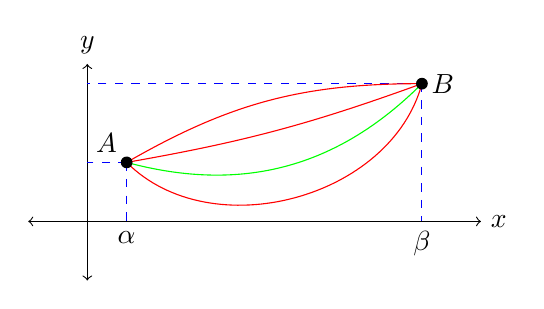
\begin{tikzpicture}
		\coordinate (origin) at (0.5,0.75);
		\coordinate (b) at (4.25, 1.75);
		
		% \filldraw[color=blue!80, fill=blue!2] (z1) circle (0.7);

		% draw axes
		\draw [<->] (-0.75, 0) -- (5.0, 0) node [right] {$x$};
		\draw [<->] (0, -0.75) -- (0, 2.0) node [above] {$y$};
	
		\draw [dashed, blue] (b) -- (4.25, 0) node [black, below] {$\beta$};
		\draw [dashed, blue] (b) -- (0, 1.75); % node [black, left] {$y_2$};

		\draw [dashed, blue] (origin) -- (0.5, 0) node [black, below] {$\alpha$};
		\draw [dashed, blue] (origin) -- (0, 0.75);

		% draw some paths between A and B
		\draw [green] (origin) to [bend right=30] (b);
		\draw [red] (origin) to [bend right=60] (b);
		\draw [red] (origin) to [bend right=5] (b);
		\draw [red] (origin) to [bend left=15] (b);

		% \draw (2.25, -0.5) node [red] {$\gamma$};
		% \draw plot [smooth, red] coordinates {(0,0) (2.0, -1.2) (4.0, -2.0))};

		% draw the points A and B
		\node at (b)[circle,fill,inner sep=1.5pt]{};
		\draw (b) node [right] {$B$};

		\node at (origin)[circle,fill,inner sep=1.5pt]{};
		\draw (origin) node [above left] {$A$};

		% draw vectors
		% \draw [->] (origin) -- (z1) node [anchor=south west] {$c$};
		% \draw [dashed] (1, 1.25) -- (0.3, 1.25) node [pos=0.5, anchor=south] {$\rho$};
		\end{tikzpicture}
\end{center}

Our strategy will be to consider some small perturbation $y \mapsto y + \epsilon \eta(x)$, where $\eta(\alpha) = \eta(\beta) = 0$. From this, we will compute $F[y + \epsilon \eta]$. To proceed with this strategy, we will need an important lemma.

\begin{lemma}[Fundamental Lemma of Calculus of Variations]
	If $g: [\alpha, \beta] \rightarrow \R$ is continuous on $[\alpha, \beta]$ and is such that
	$$
	\int_{\alpha}^{\beta} g(x) \eta(x) \dd x = 0,
	$$
	for all $\eta$ continuous on $[\alpha, \beta]$ with $\eta(\alpha) = \eta(\beta) = 0$, then $g(x) = 0$ for all $x \in [\alpha, \beta]$.
\end{lemma}
\begin{proof}
	Say (for a contradiction) that there exists some $\bar{x} \in (\alpha, \beta)$ such that $g(\bar(x)) = 0$. Say $g(\bar{x}) > 0$. Then by continuity there exists an interval $[x_1, x_2] \subset [\alpha, \beta]$ such that $g(x) > c$ on $[x_1, x_2]$ for some $c > 0$. Then set
	$$
	\eta(x) = 
	\begin{cases}
		(x - x_1)(x_2 - x) &\mbox{if } x \in [x_1, x_2], \\
		0 &\mbox{if } x \not \in [x_1, x_2].
	   \end{cases}
	$$
	Then we have
	$$
	   \int_\alpha^\beta g(x) \eta(x)) \dd x > c \int_{x_1}^{x_2} (x - x_1)(x_2 - x) \dd x > 0,
	$$
	which is a contradiction.
\end{proof}

\begin{remark}
	In the proof above, we construct a \emph{bump function} $\eta$. It is possible to make this smoother by taking various powers of the constructed function.
\end{remark}

Now let's return to our computation. We have
\begin{align*}
	F[y + \epsilon \eta] &= \int_{\alpha}^{\beta} f(x, y + \epsilon \eta, y' + \epsilon \eta') \dd x \\
	&= F[y] + \epsilon \int_{\alpha}^{\beta} \left(\frac{\partial f}{\partial y} \eta + \frac{\partial f}{\partial y'} \eta '\right) \dd x + O(\epsilon^2).
\end{align*}
We will return to the $O(\epsilon^2)$ term later, but for now we note that for an extremum of the functional, we want this first-order term to vanish, so we want something like 
$$
\left.\frac{dF[y + \epsilon]}{d\epsilon}\right|_{\epsilon = 0} = 0.
$$

We now make a move which we will return to time and time again in the calculus of variations. Integrating the $\epsilon$-term by parts,
\begin{align*}
	0 &= \int_{\alpha}^{\beta} \frac{\partial f}{\partial y} \eta - \frac{d}{dx} \left(\frac{\partial f}{\partial y'}\right) \eta \dd x + \cancel{\left[\frac{\partial f}{\partial y'}\eta\right]_{\alpha}^{\beta}} \\
	&= \int_{\alpha}^{\beta} \left(\frac{\partial f}{\partial y} - \frac{d}{dx} \left(\frac{\partial f}{\partial y'}\right)\right) \eta \dd x.
\end{align*}
Applying the fundamental lemma of the calculus of variations, we obtain the following necessary condition for an extremum.

\begin{theorem}[Euler-Lagrange Equation]
	Suppose $y \in C^2_{(\alpha, \beta)}(\R)$ is a function with fixed endpoints that extremizes the functional
	$$
	F[y] = \int_{\alpha}^{\beta} f(x, y(x), y'(x)) \dd x.
	$$
	Then $y$ must satisfy the \vocab{Euler-Lagrange} equation
	\begin{equation}\label{eq:el}
		\frac{\partial f}{\partial y} - \frac{d}{dx} \left(\frac{\partial f}{\partial y'}\right) = 0. \tag{$\dagger$}
	\end{equation}
\end{theorem}

\begin{notation}
	The LHS of the \eqref{eq:el} is denoted by $\displaystyle\frac{\delta F[y]}{\delta y(x)}$ and is the \vocab{functional derivative}.
\end{notation}

\subsection{First Integrals of the Euler-Lagrange Equations}

Of course, now that we have a necessary condition for externality, our next concern is solving the Euler-Lagrange equation.
The Euler-Lagrange equations give us a second-order ODE for $y$.
It is sometimes possible to reduce the order of the ODE to get a first-order ODE, the \vocab{first integral}, which is what we will look at in this section.

If $f$ does not explicitly depend on $y$, then $\partial f/\partial y = 0$. Then we get
$$
 \frac{d}{dx} \left(\frac{\partial f}{\partial y'}\right) = 0 \implies \frac{\partial f}{\partial y'} = c,
$$
for some constant $c$.

\begin{example}[Geodesics on the Euclidean Plane]
	Consider again the problem of finding geodesics on the Euclidean plane. 

	We want to minimize the functional
	$$
	D[y] = \int_{x_1}^{x_2} \sqrt{1 + (y')^2} \dd x.
	$$
	Using the Euler-Lagrange equations, we have $f(y') = \sqrt{1 + (y')^2}$, so $\partial f/\partial y = 0$, and thus by the result above
	$$
	\frac{y'}{\sqrt{1 + (y')^2}} = c,
	$$
	for some constant $c$. For this to be the case, we must have $y'$ constant, so $y$ is a straight line.
\end{example}


\begin{example}[Geodesics on the Sphere]
	Consider the sphere embedded in three-dimensional Euclidean space, $S^2 \subset \R^3$, and two points $A$ and $B$ on the sphere. We want to find the shortest path between $A$ and $B$.

	\begin{center}
		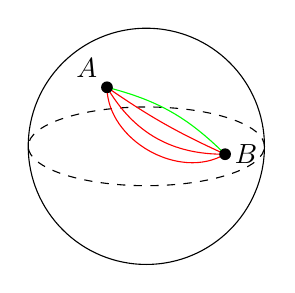
\begin{tikzpicture}
			% Draw the main 'sphere', and a great circle
			\draw (0, 0) ellipse (1.5 and 1.5);
			\draw [dashed] (0, 0) ellipse (1.5 and 0.5);

			% Pick two points on the sphere
			\coordinate (a) at (-0.5,0.75);
			\coordinate (b) at (1.0, -0.1);
			
			% draw some paths between A and B
			\draw [red] (a) to [bend right=30] (b);
			\draw [red] (a) to [bend right=60] (b);
			\draw [red] (a) to [bend right=5] (b);
			\draw [green] (a) to [bend left=15] (b);
	
			% draw the points A and B
			\node at (b)[circle,fill,inner sep=1.5pt]{};
			\draw (b) node [right] {$B$};
	
			\node at (a)[circle,fill,inner sep=1.5pt]{};
			\draw (a) node [above left] {$A$};
	
			\end{tikzpicture}
	\end{center}

	We first parameterize the sphere, with
	\begin{align*}
		x &= \sin \theta \sin \phi, \\
		y &= \sin \theta \cos \phi, \\
		z &= \cos \theta,
	\end{align*}
	where $0 < \theta \leq \pi$ and $0 \leq \phi \leq 2 \pi$. Then to find lengths of paths on the sphere, we use the line element
	$$
	\dd s^2 = \dd x^2 + \dd y^2 + \dd z^2 = \dd \theta^2 + \sin^2 \theta \dd \phi^2.
	$$
	Now we can parameterize a curve by thinking of $\phi$ as a function of $\theta$. Then we have
	$$
	\dd s = \sqrt{1 + \sin^2 \theta \cdot (\phi')^2} \dd \theta.
	$$
	Thus the functional we want to extremize is
	$$
	F[\phi] = \int_{\alpha}^{\beta} \sqrt{1 + \sin^2 \theta \cdot (\phi')^2} \dd \theta.
	$$
	We note here that $\partial f/ \partial \theta = 0$, so using the result we obtained above, $\partial f/\partial \phi' = \kappa$, for some constant $\kappa$. That is,
	$$
\frac{\sin^2 \theta \cdot \phi'}{\sqrt{1 + \sin^2 \theta \cdot (\phi')^2}} = \kappa.
	$$
	Squaring this and solving for $(\phi')^2$, we get\footnote{There is a sign ambiguity, corresponding to going either forwards or backwards around the sphere.}
	$$
	\phi'^2 = \frac{\kappa^2}{\sin^2 \theta \cdot (\sin^2 \theta - \kappa^2)} \implies \phi = \pm \int \frac{\kappa^2}{\sin^2 \theta \cdot (\sin^2 \theta - \kappa^2)} \dd \theta.
	$$
	From here, we can take a substitution of $\cot \theta = u$ to obtain the equation of a the shortest (and longest) paths.
\end{example}

Now consider, for general $f(x, y, y')$,
\begin{align*}
	\frac{d}{dx} \left(f - y' \frac{\partial f}{\partial y'}\right) &= \frac{\partial f}{\partial x} + y' \frac{\partial f}{\partial y} + \cancel{y'' \frac{\partial f}{\partial y'}} -\cancel{ y'' \frac{\partial f}{\partial y'}} - y' \frac{d}{dx}\left(\frac{\partial f}{\partial y'}\right) \\
	&= y' \left(\frac{\partial f}{\partial y} - \frac{d}{dx} \frac{\partial f}{\partial y'}\right) + \frac{\partial f}{\partial x} \\
	&= \frac{\partial f}{\partial x},
\end{align*}
where we use the Euler-Lagrange equations.
So if $f$ instead does not depend on $x$, then $\partial f/\partial x = 0$, and
$$
f - y' \frac{\partial f}{\partial y'} = c,
$$
for some constant $c$ (this is another first integral).

\begin{example}[The Brachistochrone]
	Consider again the problem of finding the shape of a wire which gives the shortest travel time for a particle sliding along it, beginning at rest.
	
	We want to minimize the functional
	$$
	T[y] = \frac{1}{\sqrt{2g}} \int_0^{x_2} \frac{\sqrt{1 + (y')^2}}{\sqrt{-y}} \dd x,
	$$
	subject to $y(x_1) =y_1$ and $y(x_2) = y_2$. Here, $f$ does not depend on $x$ and thus we can apply the result above to get 
	$$
		\frac{\sqrt{1 + (y')^2}}{\sqrt{-y}} - y' \frac{y'}{\sqrt{1 + (y')^2} \sqrt{-y}} = \kappa,
	$$
	for some constant $\kappa$. We can solve this differential equation by simplifying to get
	$$
	\frac{1}{\sqrt{1 + (y')^2}} = \kappa \sqrt{-y},
	$$
	and then we can separate variables to get
	$$
	x = \pm \kappa \int \frac{\sqrt{-y}}{\sqrt{1 + \kappa^2 y}} \dd y.
	$$
	The substitution $y = -\frac{1}{\kappa^2} \sin^2 \frac{\theta}{2}$ then gives (after some algebra)
	$$
	x = \pm \frac{1}{\kappa^2}(\theta - \sin \theta) + C,
	$$
	for some constant $C$. Using the initial conditions, we get $C = 0$, and thus
	$$
	\left\{\begin{array}{l}
		x=\frac{\theta-\sin \theta}{2 \kappa t} \\
		y=-\frac{1}{\kappa^{2}} \sin ^{2}\left(\frac{\theta}{2}\right)
		\end{array}\right.
	$$
	This is the parameterized equation of a Cycloid, the curve traced by a point on a wheel moving with constant velocity.
\end{example}


\subsection{Fermat's Principle}

We can now look at the first variational principle in this course, which describes the motion of light.

\begin{law}[Fermat's Principle]
Light travels along paths between two points which requires the least time.
\end{law}

Suppose we had a ray with path $y = y(x)$, and suppose the speed of light at $(x, y)$ is $c(x, y)$. Then we want to extremize the functional
$$
F[y] = \int \frac{1}{c} \dd s = \int_{\alpha}^{\beta} \frac{\sqrt{1 + (y')^2}}{c(x, y)} \dd x.
$$
If we assume that $c$ depends only on $x$, then we have $\partial f /\partial y = 0$, and we can use the results of the previous section to obtain
$$
\frac{\partial f}{\partial y'} = \frac{y'}{\sqrt{1 + (y')^2} c(x)} = k
$$
for some constant $k$.

If the ray is launched at an angle $\theta_1$ upwards, then $\tan \theta_1 = y'(\alpha)$. So if $\tan \theta = y'$, the above equation implies
$$
\frac{\sin \theta_1}{c(x_1)} = \frac{\sin(\theta)}{c(x)},
$$
which is known as \emph{Snell's law} in optics.

\section{Extensions of the Euler-Lagrange Equations}

We are now going to see how the Euler-Lagrange equations can be used in settings that are not just unconstrained functional extremization.

\subsection{Euler-Lagrange Equations with Constraints}

Suppose we wanted to extremimze a functional $F[y]$ with
$$
F[y] = \int_{\alpha}^{\beta} f(x, y, y') \dd x,
$$
subject to the constraint functional
$$
G[y] = \int_{\alpha}^{\beta} g(x, y, y') \dd x = k,
$$
for a constant $k$. We are going to do this by generalizing the method of Lagrange multipliers that we introduced in \autoref{sec:lm}. We are going to extremimze the functional
$$
\Phi[y, \lambda] = F[y] - \lambda G[y].
$$
To do this, we replace $f$ in the Euler-Lagrange equations by $f - \lambda g$, to get


{\color{red} In progress.}

\end{document}
